\documentclass[
11pt,%
tightenlines,%
twoside,%
onecolumn,%
nofloats,%
nobibnotes,%
nofootinbib,%
superscriptaddress,%
noshowpacs,%
centertags]%
{revtex4}
\usepackage{ljm}
\usepackage{listings}

\lstset{
language=C++,
basewidth=0.5em,
xleftmargin=45pt,
xrightmargin=45pt,
basicstyle=\small\ttfamily,
keywordstyle=\bfseries\underbar,
numbers=left,
numberstyle=\tiny,
stepnumber=1,
numbersep=10pt,
showspaces=false,
showstringspaces=false,
showtabs=false,
frame=trBL,
tabsize=2,
captionpos=t,
breaklines=true,
breakatwhitespace=false,
escapeinside={\%*}{*)}
}

\begin{document}

\titlerunning{dataflow processor emulator}
\authorrunning{Shabanov et al.}

\title{Features of Dataflow Processor Emulator Implementing}

\author{\firstname{B.~M.}~\surname{Shabanov}}
\email[E-mail: ]{shabanov@jscc.com}
\affiliation{Joint Supercomputer Center of the Russian Academy of Sciences -- branch of Scientific Research Institute of System Analysis of the Russian Academy of Sciences, Leninsky prospect 32a, Moscow, 119334, Russia}

\author{\firstname{E.~A.}~\surname{Kuznetsova}}
\email[E-mail: ]{mrallis@jscc.com}
\affiliation{Joint Supercomputer Center of the Russian Academy of Sciences -- branch of Scientific Research Institute of System Analysis of the Russian Academy of Sciences, Leninsky prospect 32a, Moscow, 119334, Russia}

\author{\firstname{A.~A.}~\surname{Rybakov}}
\email[E-mail: ]{rybakov.aax@gmail.com}
\affiliation{Joint Supercomputer Center of the Russian Academy of Sciences -- branch of Scientific Research Institute of System Analysis of the Russian Academy of Sciences, Leninsky prospect 32a, Moscow, 119334, Russia}

\author{\firstname{S.~S.}~\surname{Shumilin}}
\email[E-mail: ]{shumilin@jscc.com}
\affiliation{Joint Supercomputer Center of the Russian Academy of Sciences -- branch of Scientific Research Institute of System Analysis of the Russian Academy of Sciences, Leninsky prospect 32a, Moscow, 119334, Russia}

\firstcollaboration{(Submitted by S.~S.~Submitter)}

\received{May 01, 2020}

\begin{abstract}
The development of dataflow processor architecture is a promising direction for improving the performance of computing systems.
The dataflow processors have several advantages in contrast with the von Neumann architecture processor.
These advantages are express in explicit parallelism of calculations, since in the presentation of programs for the dataflow processors the sequence of instructions limited solely by the fact of input data’s ready state.
The concept of using tokens as data storage for instructions allows you to remove many problems associated with data conflicts and simplifies the program logic.
One of the most important elements in the implementation of the logic of the dataflow processor is the content-addressable token memory, which should provide storage and quick search for ready-made data for instructions that can be transferred for execution.
This article discusses the functionality of the dataflow processor emulator and its parts including content-addressable token memory and the logic of its operation using the example of a simple dataflow graph.
\end{abstract}

\subclass{68N20,68R10} % Enter 2010 Mathematics Subject Classification.

\keywords{Dataflow processor emulator, dataflow graph, token, token state, associative memory, control flow graph, def-use graph.}

\maketitle

\section{Introduction}

The processor with dataflow architecture (the dataflow processor) has the potential to provide the highest performance among processors because of parallelism of program execution laying down since the program graph created.
Thereby performance is not required to be detected using sophisticated equipment from the sequence of instructions specified by the instruction counter, as is the case in a processor with the von Neumann architecture.
A program in the dataflow processor is the oriental graph where nodes are instructions and information transfers by the edges as tokens, which contains the data field and context field of transferring data.
This context identifies where token should transfers (the number of receiver command in the graph) and also contains the number of an index, iteration, and the subprogram execution, which allow executing different iterations of inner cycles and different executions of procedures at the same program graph at parallel.
Regardless of the place of the two-input instruction in the graph, it transfers for execution upon arrival at the input of the last of the pair of operand tokens with the same context.
After the execution, the result in the actuator, new tokens with the result value sends to the inputs of subsequent commands according to the program column, and the used operands destroy.

At the same time, in contrast to the von Neumann architecture, the dataflow processor has not a central control device (instruction counter), and the parallelism of the executing instructions determined in dynamics by the arrival of operands to the instruction inputs in the decentralized scheme.
Namely, the device for searching ready-to-execute commands -- the memory of searching pairs (the content-addressable memory) can be executed such as many parallel-running modules, which provides the same large numbers of actuators. Since the execution of an instruction is dependent upon the arrivals of operands, the management of token storage and instruction scheduling are intimately related in any dataflow computer \cite{fine-grained-prl,culler}.

Unlike the implementation of a multiprocessor system, direct hardware implementation allows you to fully implement the calculation graph in the form of a computing pipeline, thereby eliminating the need to create a module that implements the execution of the calculation schedule \cite{popov}.

The difficulties noted above for the hardware implementation of the dataflow processor led to the fact that none of the many projects for its creation was possible to achieve higher performance compared to the von Neumann processor, and by the end of the 2000s, there were practically no such projects.
This refers to the development of universal dataflow processors, but not specialized ones, since, for example, dataflow processors of digital signal processing were not only developed, but also produced \cite{terada}.

The Joint Supercomputer Center of the Russian Academy of Sciences (JSCC RAS) is developing a vector processor with the dataflow architecture \cite{vpp}. This paper introduces the development of the emulator of the model of this processor. 


\section{Emulation of processor with the von Neumann architecture}

One of the basic principles of the von Neumann architecture is the principle of control flow.
According to it, the executable code of the program is stored in memory, and the processor can execute its instructions sequentially, one by one.
The next instruction address submitted to the processor for execution is stored in a special register called instruction pointer.
By default, it always shifts to the next instruction in memory.
This address can be forcedly changed by special transition instructions, and in this case, we can talk about transferring control to another part of the program.

Let's introduce the concept of a linear section (or program basic block).
The linear section is a sequence of instructions with the next two properties.
First, control could only be transfer to the first instruction of a given section.
In other words, a linear section has only one input, which is the section's first  instruction.
Second, if control was transferred to the linear section, than all instructions of this section must be executed (i.e., there can be no transition instructions inside the linear section).
The transition instruction can only be at the end of the linear section.
Sometimes, instead of linear sections, it is convenient to view so-called quasilinear sections, which can have an arbitrary amount of transition instructions inside for transitions to other linear sections.
We will not review quasilinear sections, because any such section can be split into a sequence of ordinary linear sections.

An important concept widely used in the theory of optimizing compilers is the control flow graph (CFG) \cite{Muchnick}.
A control flow graph is a directed graph whose nodes are linear sections of the program, and edges indicate the transfer of control between them.
The control flow graph is a convenient and demonstrative structure for describing program behavior and used by optimizing compilers to implement global program optimizations i.e. optimizations that go beyond linear sections.

Consider the logic of intermediate program representation inside one linear section.
Consider for this a simple example of finding the roots of a quadratic equation.
We will use listing in the C programming language to write examples and pseudocode.
Thus, we have a linear section (program code block) at the input of which we have the variables $a$, $b$, $c$ containing the coefficients of the quadratic equation $ax^2 + bx + c = 0$.
At the linear section output it is required to get the values of the roots, which are calculated by the formulas $x_{1,2} = (-b \pm \sqrt{b^2 - 4ac})/(2a)$.

\begin{lstlisting}[caption={The code block for calculating the roots of quadratic equation.},label={lst:square_equation_1}]
{
    float t = sqrt(b * b - 4.0 * a * c);
    
    x1 = (-b + t) / (2.0 * a);
    x2 = (-b - t) / (2.0 * a);
}
\end{lstlisting}

\

In listing~\ref{lst:square_equation_1}, the linear section is highlighted by curly brackets and temporary variable $t$ is declared to understand that this variable is not used outside the linear section.
For convenience, we assume that the processor, for which the executable code will be created, supports the instruction for calculating the square root.
Thus, the following instructions for working with real numbers appear in the listing above: MUL -- multiplication of two numbers, SUB -- subtraction of two numbers, SQRT -- the square root of a number, NEG -- unary negative, ADD -- addition of two numbers, DIV -- division of two numbers.

\begin{figure}[h]
\setcaptionmargin{5mm}
%\onelinecaptionsfalse % if the caption is multiline
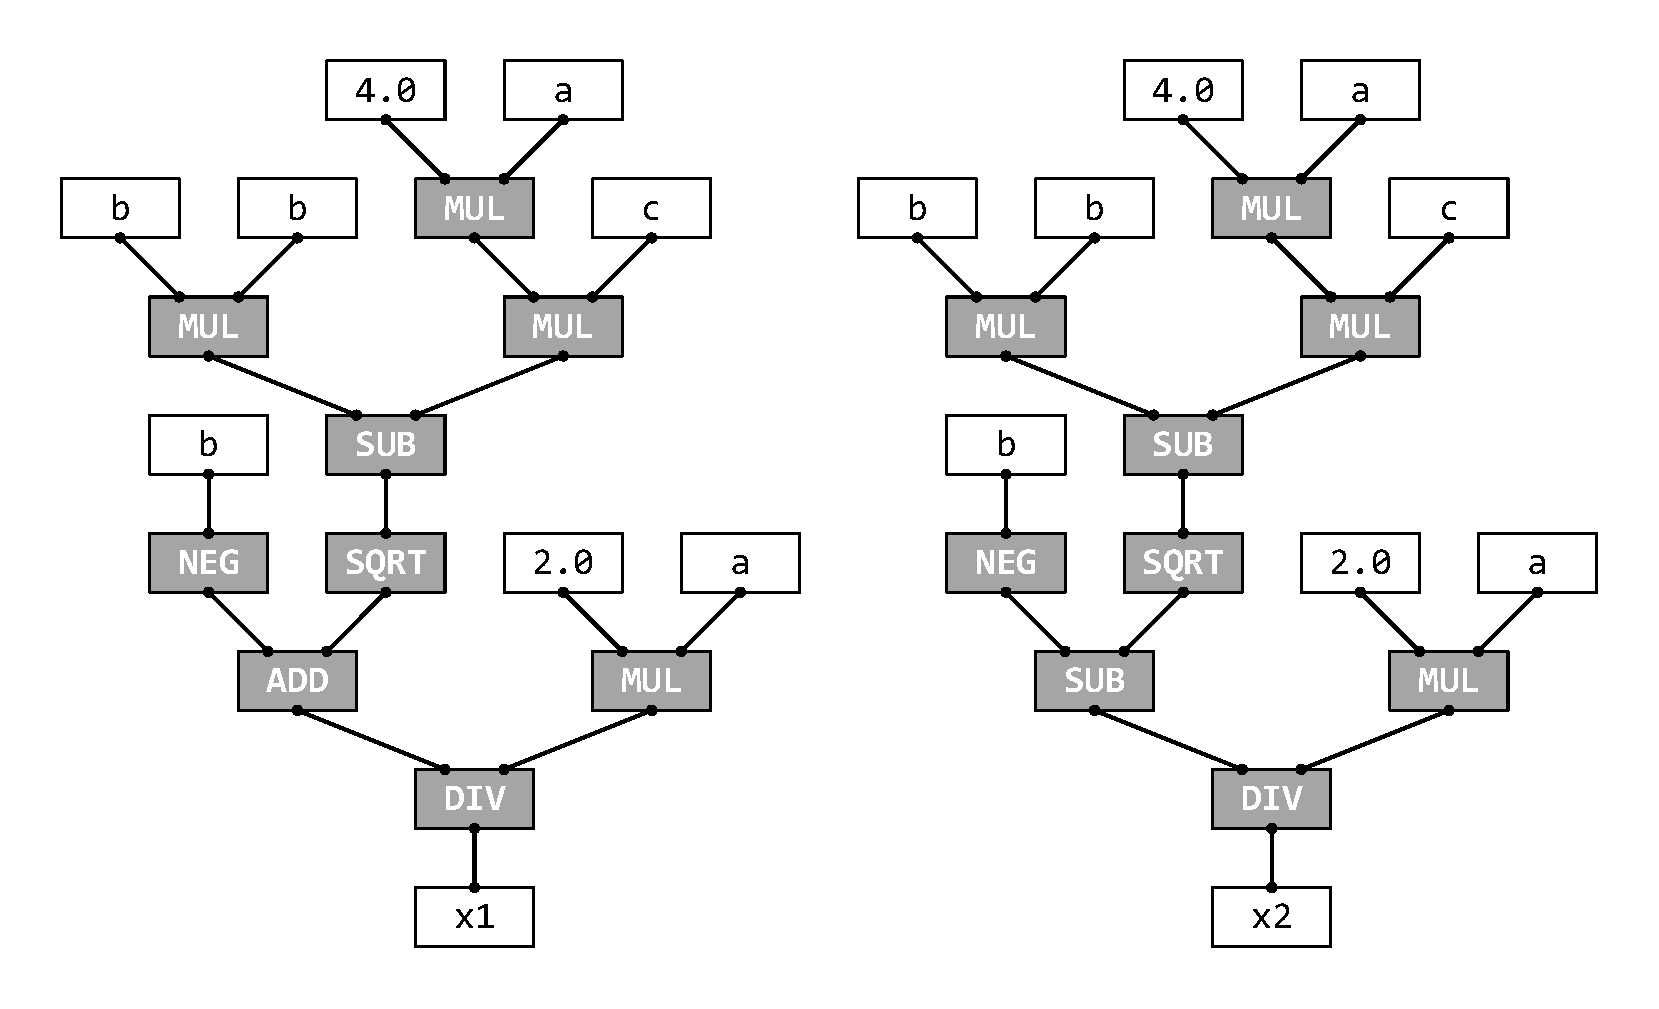
\includegraphics[width=0.95\textwidth]{pics/square_equation_calculation_tree.pdf}
\captionstyle{normal}\caption{Tree for calculating the expressions of the roots of the quadratic equation.}\label{fig:square_equation_calculation_tree}
\end{figure}

Figure~\ref{fig:square_equation_calculation_tree} shows two trees of evaluating the expressions $x_1$ and $x_2$.
The compiler, of course, will simplify the calculation data by collecting common subexpressions, and the final version of the linear section representation will be close to the next dependency graph shown in Figure~\ref{fig:def_use} (def-use graph, DFG).

\begin{figure}[h]
\setcaptionmargin{5mm}
\onelinecaptionsfalse % if the caption is multiline
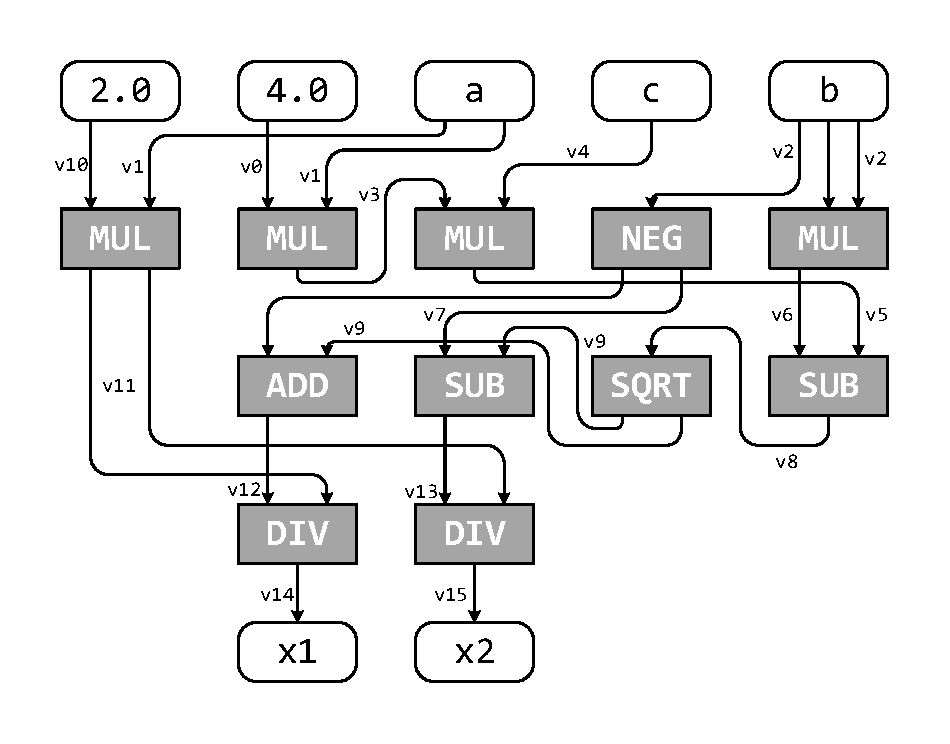
\includegraphics[width=0.60\textwidth]{pics/def_use.pdf}
\captionstyle{normal}\caption{The dependency graph of the linear section in the calculation \\ of expressions of quadratic equation's roots.}\label{fig:def_use}
\end{figure}

Nodes of this directed graph are separate operations (shown as dark rectangles), and edges are def-use dependencies between data operations (the $B$ command depends on the data from the $A$ command if uses the data generated by the $A$ command).
It can be another dependency between operations besides data dependency (control dependency, anti-dependency), but these dependencies are missing in our simple example.

To form the resulting executable code the presence of a def-use graph is not enough.
It is necessary to line up all commands included in the def-use graph in a single sequence, which will subsequently be written to a linear section of memory.
In this case, when aligning a sequence of commands, it is necessary to observe the requirement that if the $B$ command depends on the $A$ command according to the data, then it should be later than the $A$ command in the final sequence.
This process called code planning \cite{Aho}.
In the result of code planning in the considered case, we will get a pseudocode for calculating the roots of quadratic equation similar to one in listing~\ref{lst:square_equation_2}.

\begin{lstlisting}[caption={Pseudocode for calculating the roots of  quadratic equation.},label={lst:square_equation_2}]
MOV 4.0       ->  v0
MOV   a       ->  v1
MOV   b       ->  v2
MUL  v0,  v1  ->  v3
MOV   c       ->  v4
MUL  v3,  v4  ->  v5
MUL  v2,  v2  ->  v6
NEG  v2       ->  v7
SUB  v6,  v5  ->  v8
SQRT v8       ->  v9
MOV 2.0       -> v10
MUL v10,  v1  -> v11
ADD  v7,  v9  -> v12
SUB  v7,  v9  -> v13
DIV v12, v11  -> v14
DIV v13, v11  -> v15
MOV v14       ->  x1
MOV v15       ->  x2
\end{lstlisting}

\

In listing~\ref{lst:square_equation_2}, all instructions except transmission operation operate on virtual registers (v0-v15).
The order of the commands is important in this form.
At any time after the execution of any instruction, we can talk about some state of the processor which is characterized by the content of memory and of all the registers used.

The main part of the processor emulator is the realization of instruction semantic, executed by the processor.
Every instruction is considered as a function, which transfers computer from one state to another.

\section{Dataflow processor emulation}

The dataflow processor emulator, which considered in this article, has a dynamic model.
It permits to pass the commands for execution when their tokens are ready with the simultaneous execution possibility of inner cycle’s iterations and different procedure launches on the same program graph.

The dynamic model of the dataflow processor allows revealing more parallelism in program due to not only the coincidence of command number of the operand tokens, but also several fields, for example, index number, iteration, and subroutine start \cite{Wiley}.

In contrast with processors with the von Neumann architecture, dataflow processors lack complete orderliness in command execution.
I.e. if two instructions can be executed in parallel (this is possible in the absence of dependence between them) then the order of their execution is not determined.
We will consider the same example of the linear section, inside which the roots of the quadratic equation are calculated.
The program for the dataflow processor is the graph just like the def-use graph showed in Figure~\ref{fig:def_use}.
Dataflow graph, which is a program for dataflow processor, is also oriented.
The nodes of this graph also are the instructions, but edges have a completely different meaning.
In the case of def-use graph, edges were fixed fact of the dependence between two operations (indicating by which variables, by which resource), in case of dataflow graph the edge is a unique data carrier that names token.
Therefore, the token is a data structure that stores information about transferring data and about the destination point of this data (the identifier consuming this instruction data as well as the argument number, which this data is for the instruction).
Besides, the token contains additional information (token state) allowing to distinguish instruction, which relates to different function processes or to different loop iteration, but for this example, this is not important, therefore, the description of token state will be omitted.

\begin{figure}[h]
\setcaptionmargin{5mm}
\onelinecaptionsfalse % if the caption is multiline
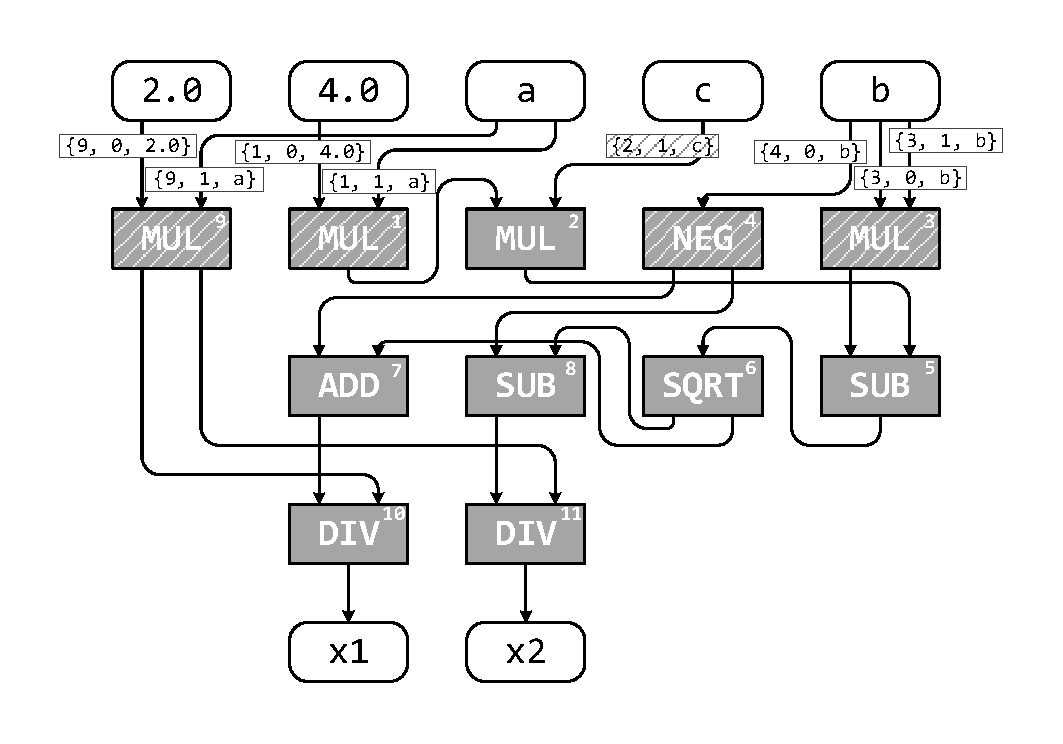
\includegraphics[width=0.80\textwidth]{pics/dataflow.pdf}
\captionstyle{normal}\caption{Dataflow graph of a linear section which calculates \\ the roots of quadratic equation.}\label{fig:dataflow}
\end{figure}

Figure~\ref{fig:dataflow} shows us the dataflow graph in the initial time when none of the instructions have been completed yet.
In this figure, on the edges of the graph, you can see those tokens that are ready and transferred to the relevant instructions.
For example, for the instruction 9 MUL two tokens are ready: $\{9, 0, 2.0\}$ (9 -- number of instruction, 0 -- number of argument, 2.0 -- real number), $\{9, 1, a\}$ (9 -- number of instruction, 1 -- number of argument, $a$ -- real number).
Both arguments for the instruction 9 MUL are ready and instruction can be executed.
After execution, tokens containing arguments are deleted, and tokens containing the result of instruction 9 MUL will be sent by the output edges to instructions 10 DIV and 11 DIV.

If we consider another instruction 2 MUL, we can see that only the second argument is ready for it (token $\{2, 1, c\}$).
The first argument will only be generated after executing the 1 MUL instruction.

Thus, all instructions in the presented graph will be processed until the required values are obtained in tokens on the output edges from instructions 10 DIV and 11 DIV.

The implementation of instruction semantics in a dataflow processor emulator is no different from the same functionality in a traditional processor emulator.

The central functional element for ensuring the operability of the dataflow processor is so-called associative token memory, the implementation of which is the purpose of this article.

Associative token memory is a repository of tokens that are currently created and are being executed in the program.
Moreover, if it turns out that in the associative memory there are all the necessary arguments for a command, they are immediately removed from the associative memory and sent for execution to the command.
Thus, at any moment in time in the associative memory there are only those arguments that wait for the missing arguments for some instructions.
That is, at the conditionally first moment in time, shown in the figure~ \ref{fig:dataflow}, in the associative memory of tokens there is only one token $\{2, 1, c\}$, waiting for its pair, while the commands are 9 MUL, 1 MUL, 4 NEG, 3 MUL are already ready for execution and are in the command buffer along with sets of their arguments.

The dataflow processors approach resolves any threads of control into separate instructions that are ready to execute as soon as all required operands available \cite{silc}. 
In the figure ~\ref{fig:dataflow} the token located in the associative memory is shaded, as well as the commands ready to be executed.

\begin{figure}[h]
\setcaptionmargin{5mm}
\onelinecaptionsfalse % if the caption is multiline
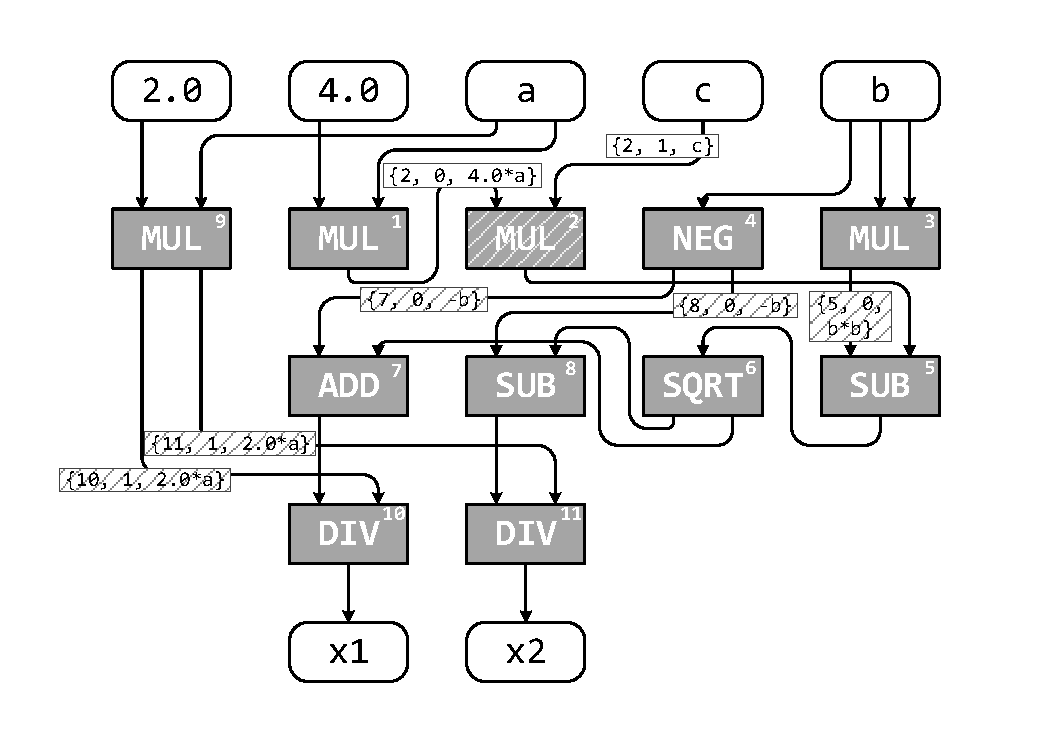
\includegraphics[width=0.80\textwidth]{pics/dataflow2.pdf}
\captionstyle{normal}\caption{Dataflow graph of a linear section which calculates the roots of quadratic equation before executing the 2 MUL instruction.}\label{fig:dataflow2}
\end{figure}

After execution of the instructions 9 MUL, 1 MUL, 4 NEG and 3 MUL, the only instruction ready for execution is 2 MUL.
The state of the computer before executing this instruction is shown in the figure ~\ref{fig:dataflow2}.
In this figure, the 2 MUL instruction ready for execution is visible, as well as several tokens that have been passed into associative memory.
Further execution of the program is similar and at the end we come to the formation of two tokens on the output edges of operations 10 DIV and 11 DIV, which will then be sent to their consumer instructions..

In the same processors, overflow of the associative memory is unacceptable, that is why the associative memory must have high capacity and be fast at the same time, which is difficult to realize into practice.
That is the point to implement the emulator, which will help to get closer to creating such the dataflow processor while revealing all possible errors and shortcomings.

\section{Architecture of dataflow processor emulator}

Consider the architecture of the dataflow processor emulator in general, presented in Figure~\ref{fig:big-scheme}.

\begin{figure}[h!]
\setcaptionmargin{5mm}
\onelinecaptionsfalse
\center{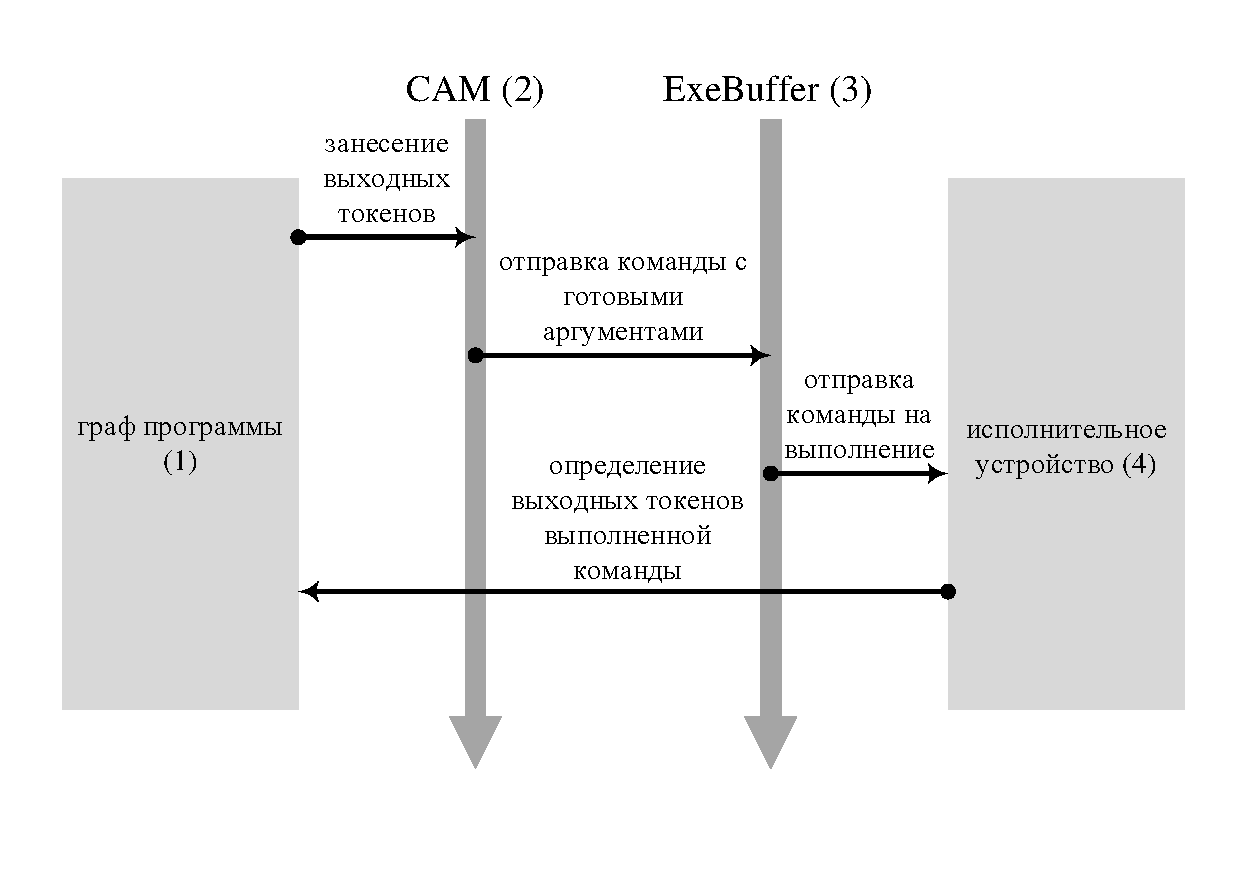
\includegraphics[width=0.80\textwidth]{pics/big-scheme.pdf}}
\captionstyle{normal}\caption{General architecture of a dataflow processor.}
\label{fig:big-scheme}
\end{figure}


Consider the main objects presented in Figure~\ref{fig:big-scheme}. Number 1 is the program, which is the input data for the emulator and presented in the form of a directed graph. Number 2 is the process serving the content-addressable token memory, which serves to collect the individual command's arguments. Number 3 is a buffer (a queue) of ready-made commands that can transfer for execution. Number 4 indicates the actuator, which in the scheme is not divided into scalar and vector. Between the described objects, the following interaction options are provided.

At the first moment, the input tokens (which can be form before the instructions execution) are determined by the program graph, these tokens are received in the CAM. The process serving the CAM runs continuously. As soon as a set of tokens found inside CAM, which is a complete set of arguments for the command, this command immediately sent to the buffer of commands ready for execution. The process serving the executive buffer also runs continuously. Its only task is to send commands from the buffer one by one for execution. After the next command executed on the actuator, the output tokens of this command determined (using the program graph) and then these tokens again transferred to the CAM. This cycle of information exchange between the elements of the emulator continues until the program shutdown command will execute. Thus, the architecture of the dataflow processor described in terms of individual processes that interact with each other through messaging. At the same time, the emulator does not have a global state, which corresponds to the ideology of the dataflow processor. Erlang programming language \cite{Armstrong,Cesarini} was chosen to implement the dataflow processor emulator.

Erlang programming language is a functional language designed to implement separate parallel processes that exchange messages. Messaging between processes is the only way to ensure communication between processes (the language does not have the concept of shared memory) it is supported at the syntactic level. Parallel to the execution of processes is a natural behavior of the language; therefore, it is not necessary to implement additional tools to ensure the interaction of system elements.

If we consider the elements of a dataflow processor emulator, then the implementation of the content-addressable token memory of particular interest. The implementation of the actuator does not fundamentally differ from the implementation in the emulator of the classical processor (the implementation of the semantics of instructions that create output tokens using input tokens). The buffer of commands ready for execution is simply a queue of commands, so its implementation is also trivial. Consider the implementation of a key element of the dataflow processor -- content-addressable token memory.

\begin{lstlisting}[caption={Implementation of the logic of the contest-addressable token memory.},label={lst:assoc}]
set_token({CId, E, _} = T, Args, D) when (Args > 1) ->
	FullEntries = lists:seq(0, Args - 1, 1),
	ET = {E, T},
	case dict:find(CId, D) of
		error ->
			dict:append(CId, ET, D);
		{ok, Vs} ->
			{Es, Ts} = lists:unzip(lists:sort(Vs ++ [ET])),
			case Es of
				FullEntries ->
					{Ts, dict:erase(CId, D)};
				_ ->
					dict:append(CId, ET, D)
			end
	end.
\end{lstlisting}

At Listing~\ref{lst:assoc} there is the compact logic implementation of content-addressable token memory in the Erlang programming language.
All the logics realize with one function $set\_token$ with three arguments: $T$ -- added token (which consists of the instructions identifier $CId$, number of argument $E$, and dates), $Args$ -- the number of arguments of the instruction for which the token is added, $D$ -- dictionary which token content-addressable memory is implemented.
The function logic turns to the next: to extract from the dictionary all the tokens, which are associated with the key $CId$, and check if they close all the arguments of considered instruction (i.e. numbers of the arguments form a sequence $[0, 1, .. Args - 1]$.).
If the added token is the last missing argument of the considered instruction, then we need to extract all the tokens from the dictionary and return them back in the form of a list for executing the instruction (line 11).
Otherwise, token should be added in the dictionary tying it to a key $CId$ (lines 6 and 13).

Note that the most simplified implementation is given.
It is not considered the possibility of using the token state for instructions identify from different function calls or from different cycles iteration (for completeness as a key of dictionary together with instruction identifier $CId$ should also use the token state).
In the given implementation, exception handling also is not considered.
For example, the sequential addition of two tokens in the content-addressable memory that is the same argument of the same instruction should cause the error.
However, despite the incompleteness of implementation, it shows here logic allows providing the functionality of the content-addressable token memory, which needed for execution of the dataflow processor’s program.

In the dataflow processor, communication between two instructions is much quicker if these instructions are allocated to the same processing element.
Thus a program may run much faster if its instructions are clustered to minimize communication traffic between clusters and each cluster is allocated to one processing element.
Since it will be handling significantly less packet traffic, the communication network of the dataflow processor will be simpler and less expensive than the distribution network in the cell block architecture.
Depending on the area of application, the technology of fabrication, and the time frame under consideration, the reduction in additional programming costs may not be justified \cite{Dennis}.

\section{Conclusion}

The article discusses the differences in the implementation of an executable program designed for a processor with von Neumann architecture and a dataflow processor.
The differences between the use-define graph and the dataflow graph are shown, which reflect the program logic within the linear section.
The necessary element of dataflow processor’s realization shown -- content-addressable token memory with which can storage and quick search the ready-made tokens for the commands, which may transfer for execution.
A compact implementation of the content-addressable token memory for instructions with an arbitrary number of iterations is given.
That realization can be expanded for any program for the dataflow processor including which use cycles and function calls (including recursive).
This approach to organizing of the content-addressable token memory used in the implementation of the vector processor with dataflow architecture emulator, which is developing at the JSCC RAS.

\begin{acknowledgments}
The work has been done at the JSCC RAS as part of the state assignment for the topic 0065-2019-0016 (reg. no. AAAA-A19-119011590098-8).
The supercomputer MVS-10P, located at the JSCC RAS, was used for calculations during the research.
\end{acknowledgments}

\begin{thebibliography}{99}

\bibitem{fine-grained-prl}
\refitem{article}
N.~A.~Dikarev, B.~M.~Shabanov, A.~S.~Shmelev, {\it ``The use of fine-grained parallelism in dataflow processor"}, Problems of developing promising micro- and nanoelectronic systems (MES), {\bf 2}, pp.~144--150 (2016).

\bibitem{culler}
\refitem{book}
D.~Culler, {\it ``Dataflow Architecture"}, MIT/LCS/TM-294, Massachusetts Institute of Technology (1986).

\bibitem{popov}
\refitem{article}
R.~I.~Popov, {\it ``Application of stream computer models in designing specialized processors."}, Scientific and Technical Journal of Information Technologies, Mechanics and Optics, {\bf 5}(75), pp.~77--81 (2011).

\bibitem{terada}
\refitem{article}
H.~Terada, {\it ``DDMP’s: Self-Timed Super-Pipelined Data-Driven Multimedia Processors."}, Proceedings of the IEEE, {\bf 2}(86), pp.~282--296 (1999).

\bibitem{vpp}
\refitem{article}
N.~A.~Dikarev, B.~M.~Shabanov, {\it ``Vector dataflow processor"}, IZVESTIYA SFedU, {\bf 10}(54), pp.~80--85 (2005).

\bibitem{Muchnick}
\refitem{book}
S.~S.~Muchnick, {\it ``Advanced Compiler Design \& Implementation."}, Academic Press (1997).

\bibitem{Aho}
\refitem{book}
A.~V.~Aho, M.~S.~Lam, R.~Sethi, J.~D.~Ullman, {\it ``Compilers. Principles, Techniques, \& Tools."}, Addison-Wesley (2007).

\bibitem{Wiley}
\refitem{book}
J.~Wiley, {\it ``Dataflow Computers: Their History and Future. \& Wiley Encyclopedia of Computer Science and Engineering, edited by Benjamin War"}, John Wiley and Sons, Inc (2008).

\bibitem{silc}
\refitem{book}
J.~Silc, B.~Robic, T.~Unqerer, {\it ``Processor Architecture: From Dataflow to Superscalar and Beyond"}, Springer Science and Business Media, (2012).

\bibitem{Armstrong}
\refitem{book}
J.~Armstrong, {\it ``Programming Erlang. Software for a Concurrent World."}, Pragmatic Programmers (2013).

\bibitem{Cesarini}
\refitem{book}
F.~Cesarini, S.~Thompson, {\it ``Erlang programming."}, O'Reilly (2009).

\bibitem{Dennis}
\refitem{article}
J.~B.~Dennis, {\it ``Data Flow Supercomputers."}, MIT Laboratory for Computer Science, {\bf 13}, pp.~48--56 (1980).

\end{thebibliography}

\end{document}
